\documentclass[12pt]{article}

\usepackage{xspace}
\usepackage{lineno}
\usepackage{setspace}
\usepackage{graphicx}
\usepackage{subfigure}
\usepackage{float}
\usepackage{color}
\usepackage{caption}
\usepackage[margin=1in]{geometry}
\usepackage{epstopdf}
\usepackage{natbib}

\begin{document}
\doublespacing
\linenumbers

\newcommand{\kluyveri}{\textit{L. kluyveri}\xspace}


\noindent RH: LANDERER ET AL.--- Intragenomic variation in codon usage
% put in your own RH (running head)
% for POVs the RH is always POINT OF VIEW
\bigskip
\medskip
\begin{center}

% Insert your title:
\noindent{\Large \bf Differences in Codon Usage Bias between genomic regions in the yeast \textit{Lachancea kluyveri}.}
\bigskip

% We don't use a special title page; the author information is entered
% like any other text.

% FOOTNOTES: We don't allow them in the manuscript, except in
% tables. Don't include any footnotes in the text.


\noindent{C\textsc{EDRIC} ~{L\textsc{ANDERER}}$^{1,2,*}$,
R\textsc{USSELL} {Z\textsc{ARETZKI}}$^{3}$,
\textsc{AND}
M\textsc{ICHAEL} A.~{G\textsc{ILCHRIST}}$^{1,2}$}

\end{center}

\vfill

{\small
\noindent$^{1}$Department of Ecology \& Evolutionary Biology, University of Tennessee, Knoxville, TN 37996-1610\\
\noindent$^{2}$National Institute for Mathematical and Biological Synthesis, Knoxville, TN 37996-3410\\
\noindent$^{3}$Department of Business Analytics \& Statistics, Knoxville, TN ~ 37996-0532 \\
\noindent$^{*}$Corresponding author. E-mail:~cedric.landerer@gmail.com
}

\vfill
\centerline{Version dated: \today}
\vfill
\newpage


\begin{abstract}
Large efforts have been made to develop and explore models to understand intra-genomic variation in codon usage bias (CUB) and the contributions of mutation and selection to its evolution.
Comparative studies have been undertaken to further our understanding of variation in codon usage between species.
However, limited efforts have been made to understand how CUB is affected, and in return effects hybridization or introgression events between species with potentially large differences in CUB. 
In this study, we explore the CUB of \textit{Lachancea kluyveri} which has experienced a large introgression covering the whole left arm of chromosome C, affecting about 10\% of all genes.
The \kluyveri genome provides insights about the adaptation of introgressed regions to the novel genomic environment, with potentially large differences in selection for translation efficiency due to factors like tRNA availability, effective population size, or differences in mutation environment.

We analyzed the CUB of the endogenous \kluyveri genome and compared it to the CUB of the exogenous, introgressed region while separating the effects of mutation bias and selection for translation efficiency on CUB.
Our results show distinct CUB between the endogenous and exogenous regions of the \kluyveri genome.
We show that this differences can be mostly attributed to differences in mutation bias.

The introgression into the \kluyveri genome is of additional interest as the source has not yet been identified.
Given our ability to clearly distinguish CUB between the exogenous and the endogenous region we explored if CUB can identify possible candidates for the origin of the introgression.
The estimation of CUB and its separation into contributions of mutation and selection across a variety of yeasts allowed us to identify two candidates for the origin of the exogenous genes.
We used orthogonal information about synteny to validate candidates obtained by matching CUB.
\end{abstract}	



\section*{Outline}

\subsection*{Introduction}

\begin{itemize}
	\item CUB changes due to differences in mutation, selection, and drift.
	\item most studies assume only one environment for mutation, selection and drift and therefore only one codon usage.
	\begin{itemize}
		\item This assumptions can be violated for multiple reasons, like introgression/horizontal gene transfer (HGT), population bottlenecks, etc.
	\end{itemize}
	 \item Variation in CUB has previously only been studied in bacteria where HGT is common.
	\begin{itemize}
		\item HGT only transfers small amount of genes, probably with little to no impact on overall CUB.
		\item However, exogenous material can accumulate if HGT is frequent \citep{lawrence1997}.
		\item Previous studies have shown that genes with similar CUB are more likely to be transferred, potentially mitigating effects of accumulation \citep{tuller2011}.
		\item Hybridization/Introgression should have a larger impact on CUB due to the amount of material transferred, possibly affecting the outcome of a study if ignored. 
	\end{itemize}
	\item In this study, we look at \kluyveri (three key results).
	\begin{itemize}
		\item \kluyveri has experienced a recent ($55.5e10$ generations) large scale introgression \citep{friedrich2015}, clearly marked by elevated GC-content \citep{payen2009}.
		\item We expect that CUB differs between the introgressed exogenous region and the endogenous region due to the great ($13 \%$) difference in GC-content between the two regions.
		\begin{itemize}
			\item We find differences in CUB between the two regions.
			\item Taking this difference into account, we can increase our ability to extract biological information (predicting gene expression).
			\item Thanks to our ability to distinguish between effects of mutation and selection on CUB, we are able to attribute most of the difference in CUB to mutation bias.
			\item Figure \ref{fig:cub_all_aa} shows the CUB if we ignore the introgression (dotted), and for the endogenous (solid) and exogenous (dashed) respectively.
		\end{itemize}
		\item At this point, the source of the introgression has not been identified.
		\begin{itemize}
			\item Since we can clearly distinguish between the endogenous and exogenous CUB, can we use this information to find possible donor organisms?
			\item We analyzed CUB for several yeasts and found several species with similar selection for translation efficiency, and a few with similar mutation bias, but only two with high agreement in both (gossypii and dubliensis, Figure \ref{fig:corr_all_species}).
			\item We validated our findings with orthogonal information from synteny where analyzed a subset of our initial yeast set.
			\item We found several closely related species with syntenious regions, but only one species that also showed agreement in CUB allowing us to exclude dubliensis since it does not show any synteny with \kluyveri (Figure \ref{fig:synteny_species} right).
		\end{itemize}
		\item Assuming gossypii as origin for the exogenous region, we estimated a time since introgression from our estimates of mutation bias.
		\begin{itemize}
			\item Based on the two codon amino acids we estimated a time since introgression on the order of $10e8$
			\item Assuming one to eight generations per day, we are finding an introgression age between 110k and 890k years, which overlaps with a previous estimate \citep{friedrich2015}.
		\end{itemize}
	\end{itemize}
\end{itemize}

\subsection*{Results}

\begin{itemize}
	\item We compared model fits of CUB for \kluyveri with a fit where we allowed CUB to vary between the endogenous and exogenous region.
	\begin{itemize}
		\item Model selection by AIC favored varying CUB between the endogenous and exogenous region of the \kluyveri genome.
		\item Comparison of predicted protein synthesis $\phi$ of both fits with empirical estimates showed that varying CUB improved our ability to predict $\phi$ ($0.59$ vs $0.69$) (Figure \ref{fig:phi_corr_two_cond}).
		\item We also observed a decrease of the variation in estimated $\phi$ when assuming only one CUB environment.
	\end{itemize}
	\item Comparison of posterior estimate between regions (ADD FIGURE).
	\begin{itemize}
		\item The comparison estimates of mutation bias ($\Delta M$) showed that X out of $40$ parameters showed a difference in sign, meaning that different codons are favored by mutation in the two regions.
		\item We find that only TTT is favored by mutation in both regions (CHECK 4 and 6 codon AA) 
		\item The comparison estimates of selection for translation inefficiency ($\Delta \eta$) showed that X out of $40$ parameters showed a difference in sign, meaning that more of the same codons are favored by selection in both regions than in the mutation case.
	\end{itemize}
	\item The exogenous region is assumed to be a recent introgression of unknown origin \citep{friedrich2015}.
	\begin{itemize}
		\item To determine a potential origin, we estimated the number of neutral substitutions that we expect to determine how different we can the exogenous region to be from its origin.
		\begin{itemize}
			\item \citep{friedrich2015} argued that the introgression occurred about $55.5e6$ generations ago, and showed that it can be found in all studied populations.
			\item Based on the length of the exogenous region ($1e6$), the mutation rate per nucleotide ($4e-10$) and the number of generations estimated ($55.5e6$) we expect about $22k$ neutral substitutions or about $2.2 \%$ of the introgressed region.
		\end{itemize}
		\item Estimates of gene trees with a fixed topology allowed us to determine that we do not observe accelerated evolution in the exogenous region when compared to the endogenous region (Figure \ref{fig:rate_evol}).
		\item these observations combined lead us to the expectation that the exogenous region should still reflect most of its original CUB environment.
	\end{itemize}
	\item We explored CUB for several yeasts species to determine if another yeast shows similar CUB.
	\begin{itemize}
		\item Comparison of CUB parameters yielded three species with agreement ($\rho > 0.5$) in mutation bias ($\Delta M$) and $29$ species with agreement in selection bias ($\Delta \eta$) (Figure \ref{fig:corr_all_species}).
		\item Only two species, gossypii and dubliensis showed agreement in both, $\Delta M$ and $\Delta \eta$ (Figure \ref{fig:corr_all_species}).
		\item musiva showed a positive correlation in in both $\Delta M$ and $\Delta \eta$ but did not satisfy our arbitrary cutoff.
	\end{itemize}
	\item We used synteny as an independent approach as a means to validate our candidate list.
	\begin{itemize}
	\item The check if a subset of our yeast (including our two candidates) shows synteny with the exogenous region revealed eight species (Figure \ref{fig:synteny_species}).
		\begin{itemize}
			\item dubliensis, a candidate based on CUB, did not show a synteny relationship with the exogenous region.
			\item gossypii, the other candidate, was found to have a synteny coverage of $95 \%$ (Figure \ref{fig:synteny_species}).
			\item the other six yeasts with synteny showed agreement with only agreement in $\Delta \eta$ but not in $\Delta M$ (CHECK mutation/selection CORRELATION).
		\end{itemize}	 
	\end{itemize}
	\item Under the assumption that the exogenous region originated from gossypii, we estimated the time since introgression.
	\begin{itemize}
		\item For simplicity, only the two codon amino acids were used. 
		\item We again assumed a mutation rate of $4e-10$.
		\item Based on the difference in mutation bias $\Delta M$ between gosypii and the endogenous region we estimated a decay curve.
		\item knowing the current $\Delta M$ parameters allowed us to place the xogenous region on that curve, providing us with an estimate of the time since introgression of about $4e8$ generations.
		\item Assuming one to eight generations per day for \kluyveri we estimate a time since introgression of about $110k$-$890k$
		\item combining our estimates with the estimates of \citep{friedrich2015} ($19k$-$150k$) we date the age of the introgression to be between $110k$-$150k$.
		\item Our time since introgression depends on gossypii being the origin and has not changed it's CUB since the introgression occurred.
	\end{itemize}
\end{itemize}


\subsection*{Discussion}

\begin{itemize}
	\item based purely on selection, we would have not been able to identify the difference in CUB between the endogenous and exogenous region.
	\item With approaches like CAI or tAI, which are purely focused on selection we would not have been able to narrow the species down that much.
	\begin{itemize}
		\item However, in this particular case GC-content alone would have gotten us to the same result. 
		\item GC-content would be faster, but can be expected to lead to more candidates since it is a more coarse grain approach. 
	\end{itemize}
\end{itemize}


\subsection*{Materials and Methods}

\begin{itemize}
	\item \kluyveri genome preparation
	\begin{itemize}
		\item We obtained the CDS for \kluyveri from weird french site
		\item We split the CDS into two partitions, an exogenous region, describing the introgression and an endogenous partition based on \citep{payen2009}.
	\end{itemize}
	\item \kluyveri model fitting

\end{itemize}



\bibliographystyle{plain}
\bibliography{kluyveri_paper}

\section*{Figures and Tables}

\begin{figure}[H]
    \centering
    \begin{subfigure}
        \centering
        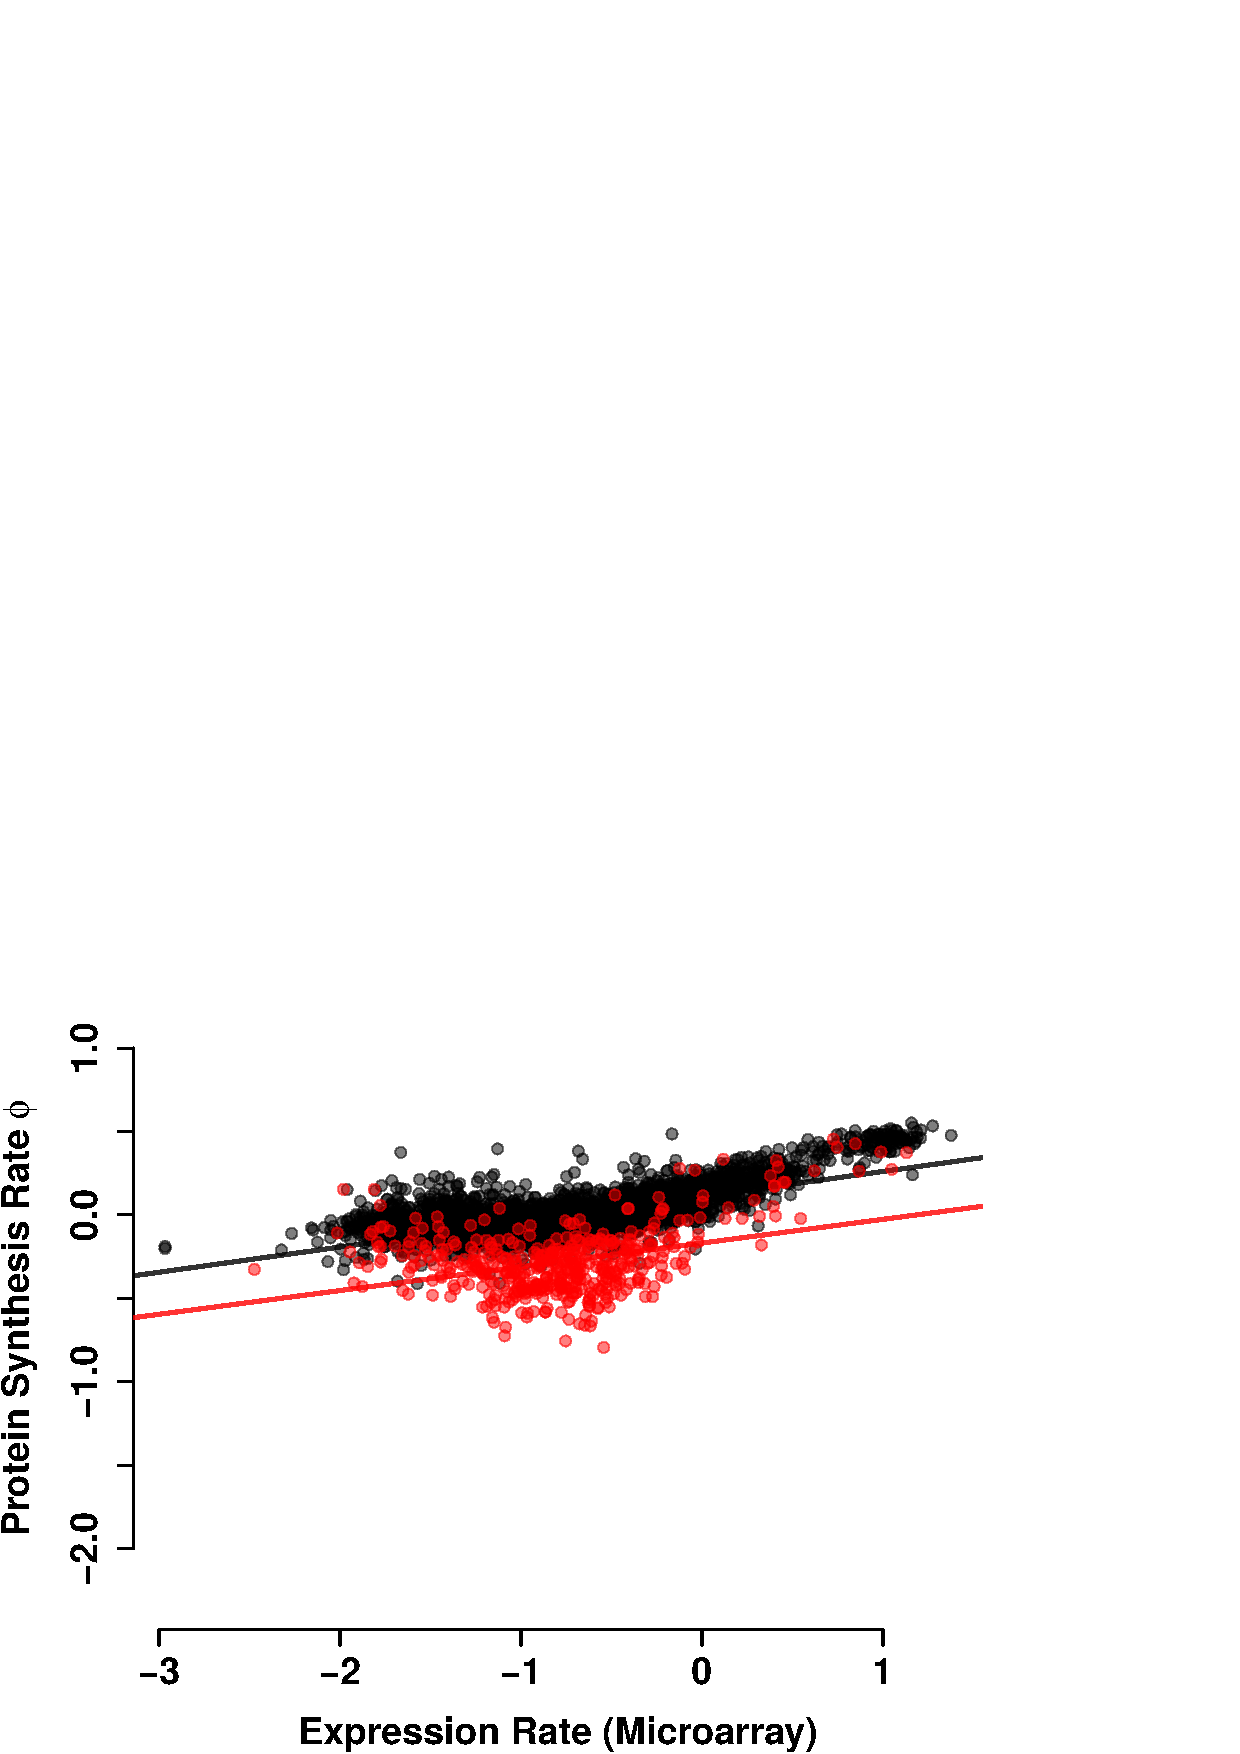
\includegraphics[width=.45\textwidth]{img/phi_corr_plot_whole_Genome_estim.pdf}
    \end{subfigure}
    \begin{subfigure}
        \centering
        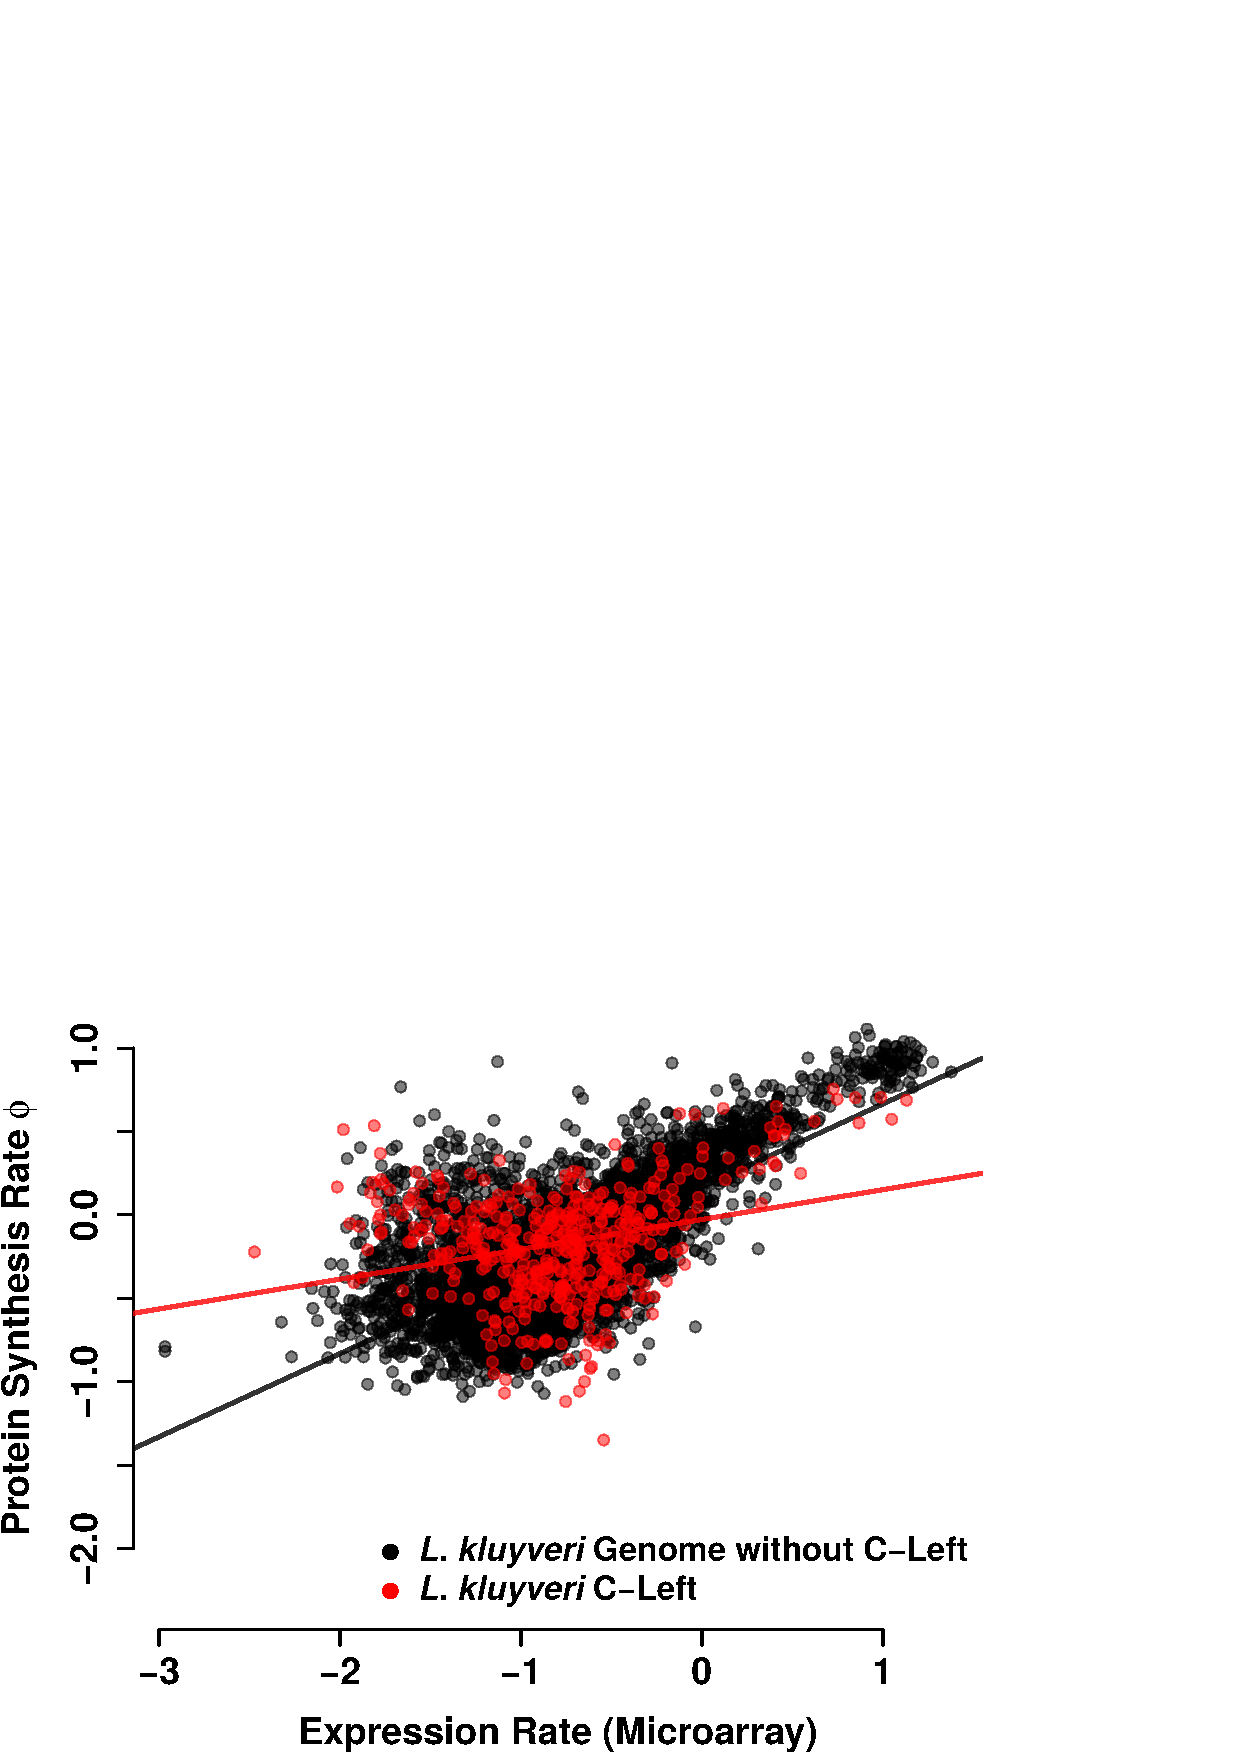
\includegraphics[width=.45\textwidth]{img/phi_corr_plot_split_Genome_estim.pdf}
    \end{subfigure}
    \caption{Person correlation of predicted protein synthesis rate $\phi$ with observed expression rate. )}
    \label{fig:phi_corr_two_cond}
\end{figure}


\begin{figure}[H]
     \centering
	\includegraphics[width=\textwidth]{img/CUB_cleft_main.pdf}
	\caption{Codon Usage}
	\label{fig:cub_all_aa}
\end{figure}

\begin{figure}[H]
     \centering
	\includegraphics[width=\textwidth]{img/rate_of_evolution.pdf}
	\caption{Overall time passed along gene tree}
	\label{fig:rate_evol}
\end{figure}

\begin{figure}[H]
     \centering
	\includegraphics[width=\textwidth]{img/csp_correlations.pdf}
	\caption{Codon Usage}
	\label{fig:corr_all_species}
\end{figure}


\begin{figure}[H]
    \centering
    \begin{subfigure}
        \centering
        \includegraphics[width=.45\textwidth]{img/synteny_blocks_and_gc.pdf}
    \end{subfigure}
    \begin{subfigure}
        \centering
        \includegraphics[width=.45\textwidth]{img/synteny_coverage.pdf}
    \end{subfigure}
    \caption{Synteny stuff}
    \label{fig:synteny_species}
\end{figure}


\end{document}








